\chapter{Matériel et Méthodes}

\section{Flux de travail}

Pour réaliser le jeu de données nécessaire à l'entrainement de notre réseau de neurone,
nous avons utilisé le site Xeno-Canto \cite{XenoCanto}. Celui-ci recense un grand nombre de chants d'oiseau
de différentes espèces enregistré par des utilisateurs.
Cependant, les chants d'oiseaux enregistrés possèdent des caractéristiques différentes (durée d'enregistrement,
format d'enregistrement, sample rate, bruit de fond).
Notre premier défi a donc été de créer un jeu de données permettant 
d'obtenir des résultats corrects. 
Pour cela, nous nous sommes fixé pour objectif d'obtenir une précision supérieure à 80\% sur les données de test
avec un réseau de neurone de type M5 \cite{M5}.
Cela nous permet entre autre de valider notre jeu de données. 
Nous avons donc suivi une approche itérative \ref{graph:iterative_workflow}

\begin{figure}[!ht]
  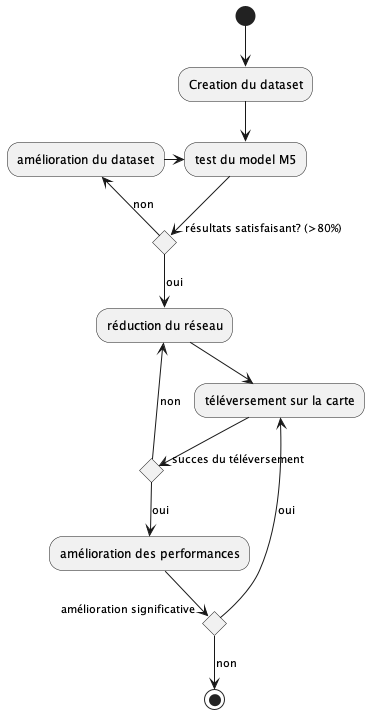
\includegraphics[width=0.5\textwidth]{iterative_workflow}
  \centering
  \caption{Workflow Iteratif}
  \label{graph:iterative_workflow}
\end{figure}

À chaque itération, nous essayer d'obtenir une meilleure précision qu'à l'itération précédente.
Notre première approche a consisté à récupérer le son de 10 espèces d'oiseaux depuis Xeno-Canto puis
à les convertir en .wav avant de tester le réseau de neurone M5 dessus.

Pour ce faire nous avons développé en script de scrapping en Python nous permettant de sélectionner les espèces 
que nous voulions télécharger depuis le site. Lors de la récupération des sons, nous avons choisi de laisser 
un délai de 1 seconde entre chaque téléchargement pour ne pas surcharger le site. Nous avons également utilisé un script 
de conversion des fichiers en wav et de resampling en 16 000 Hz. Les scripts utilisés sont disponibles sur
notre repository GitHub  \cite{Repository}.

Cette approche ne nous a malheuresement pas permit d'obtenir des résultats satisfaisant. En effet, 
le réseau de neurone M5 ne nous permettait d'obtenir qu'une précision de 20\%.

Nous avons donc choisis de découper les sons de notre jeu de données en échantillons de 1 seconde.
Ce traitement de notre jeu de données nous a permi d'obtenir une amélioration de la précision 
du réseau de neurone M5 sur notre dataset qui est passée de 20\% à 40\%. Cependant, nous pouvons 
trouver plusieurs défaut à cette approche. La principale est que sur les enregistrement de plusieurs minutes,
les chants d'oiseau ne sont pas constant et il existe des périodes de silence. 
Nous en déduisons qu'une des raisons de la mauvaise performance de notre réseau de neurone 
et que certains échantillons ne contiennent pas de chants d'oiseaux. 

Nous avons réflechis à plusieurs façon de résoudre ce problème : 
\begin{itemize}
  \item Controller manuellement la présence ou non de chant d'oiseau 
  \item Filtrer les sons automatiquement et supprimer les silences
  \item Entrainer un algorithme non supervisé pour permettre de détecter les échantillons potentiellement mal labélisés
\end{itemize}





\begin{figure}[!ht]
  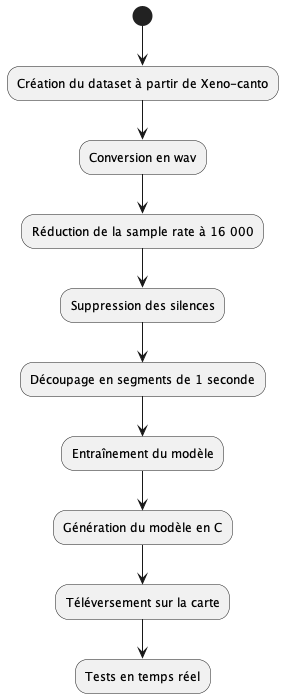
\includegraphics[width=0.5\textwidth]{final_workflow}
  \centering
  \caption{Workflow Final}
  \label{graph:final_workflow}
\end{figure}


\section{Jeu de données}
• Description of the workflow to solve the problem described before (from training to
embedded AI and communication). Add a figure illustrating that flow.
• Description of the CNN model obtained after training by taking inspiration on the first labs
• Presentation of the processing architecture of the sensor’s data
o Provide a definition of DMA and ADC


\begin{center}
  \begin{tabular}{ |c|c|c|c| }
   \hline
   \multicolumn{4}{|c|}{Jeu de données: Espèces d'oiseaux} \\
   \hline
    Nom Français & Nom Anglais & Espèce & Nombre d'échantillons\\
   \hline
    Alouette des champs & Eurasian skylark & Alauda arvensis & 3 381\\
    Bruant jaune & Yellowhammer & Emberiza citrinella & 3 278\\
    Bruant zizi & Cirl bunting & Emberiza cirlus & 3 305\\
    Coucou gris & Common cuckoo & Cuculus canorus & 3 323\\
    Effraie des clochers & Barn owl & Tyto alba & 3 254\\
    Faucon crécerelle & Common kestrel & Falco tinnunculus & 3 311\\
    Fauvette des jardins & Garden warbler & Sylvia borin & 3 398\\
    Gobemouche gris & Spotted flycatcher & Muscicapa striata & 3 319\\
    Grèbe castagneux & Little grebe & Tachybaptus ruficollis & 3 167\\
    Hirondelle de fenêtre & Common house martin & Delichon urbicum & 3 369\\
   \hline
  \end{tabular}
\end{center}

\section{Description du CNN}

\begin{center}
  \begin{tabular}{ |c|}
   \hline
    Input: 16000x1\\
   \hline
    Maxpool: 10x1 (output: 1600 × n)\\
   \hline
    conv1d [80/4, 32]\\
   \hline
    Maxpool: 4x1 (output: 100 × n)\\
   \hline
    conv1d [3, 32]\\
   \hline
    Maxpool: 4x1 (output: 25 × n)\\
   \hline
    conv1d [3, 32]\\
   \hline
    Maxpool: 4x1 (output: 6 × n)\\
   \hline
    conv1d [3, 32]\\
   \hline
    Maxpool: 3x1 (output: 1 × n)\\
   \hline
  \end{tabular}
\end{center}

\section{Architecture du traitement de données par le capteur}
